\section{Experiment 10H-E: leakage-safe innovation separability}
\label{sec:experiment10he}

\paragraph{Question and leakage constraint.}
Experiment 10H-D showed that matrices regressed from a single nominal
observer's pseudo-states are not physically comparable. Experiment 10H-E asks
the prerequisite question for a mixture-of-state-space-models approach: do
the locally measured innovation sequences already contain enough information
to distinguish compatible vehicle groups before state or matrix learning?

The grouping pipeline is deliberately leakage-safe. It never receives a
client's true mass, inertia, tire stiffness, geometry, relaxation length,
actuator constant, latent state, LPV matrix, or physical class label. Every
client uses the same fixed nominal observer specified independently in the
configuration as an engineering design prior. Its values are not the true
parameters of any client and are not adapted from fleet labels. True class
labels are opened only after unsupervised fitting for retrospective ARI,
balanced accuracy, and class-recall diagnostics.

\paragraph{Innovation signatures.}
For every locally observed speed, the client calculates
\begin{equation}
 \nu_{i,k}=y_{i,k}-C\hat x_{i,k|k-1},
 \qquad y=[r,a_y,\delta_a]^\top,
\end{equation}
using only measured outputs, steering command, and speed. The trajectory is
centered and whitened by the fixed sensor-noise covariance. The communicated
signature contains aggregate covariance, lag-one autocorrelation, normalized
innovation-energy statistics, innovation--input cross moments, and three-band
spectral energies. Raw measurements, pseudo-states, and trajectories remain
local.

Because every client covers only one speed block, known block effects are
removed using blockwise fleet means and standard deviations. PCA retains at
most eight components. Diagonal-covariance Gaussian mixtures with 24
deterministic restarts test $K\in\{1,\ldots,5\}$; BIC selects the cardinality
subject to at least five clients per group. Development uses seeds 561--570.
Confirmation seeds 571--580 remain reserved.

\paragraph{Result.}
BIC selects $K=1$ in all ten development fleets. The resulting ARI is zero and
balanced accuracy is $1/3$. The entropy gate passes trivially because a
one-group solution has no membership ambiguity; it must not be interpreted as
confident physical classification.

A retrospective fixed-$K=3$ diagnostic separates model-selection failure from
feature-separability failure. It obtains mean ARI 0.455 and mean balanced
accuracy 0.747. Results are inconsistent: two fleets reach ARI above 0.80 and
balanced accuracy 0.933, whereas several fleets completely lose one physical
class. The minimum class recall over all development fleets is zero. BIC for
$K=3$ is 24--54 points worse than for $K=1$, so the evidence for three groups
is not merely just below a selection threshold.

\begin{table}[htbp]
\centering
\caption{Experiment 10H-E development innovation-separability diagnostics.}
\label{tab:experiment10he}
\begin{tabular}{lrr}
\toprule
Diagnostic & Unknown-$K$ result & Fixed-$K=3$ diagnostic\\
\midrule
Modal selected groups & 1 & 3 fixed\\
Mean ARI & 0.000 & 0.455\\
Mean balanced accuracy & 0.333 & 0.747\\
Minimum class recall & 0.000 & 0.000\\
Fleets with ARI $>0.8$ & 0/10 & 2/10\\
\bottomrule
\end{tabular}
\end{table}

\begin{figure}[htbp]
\centering
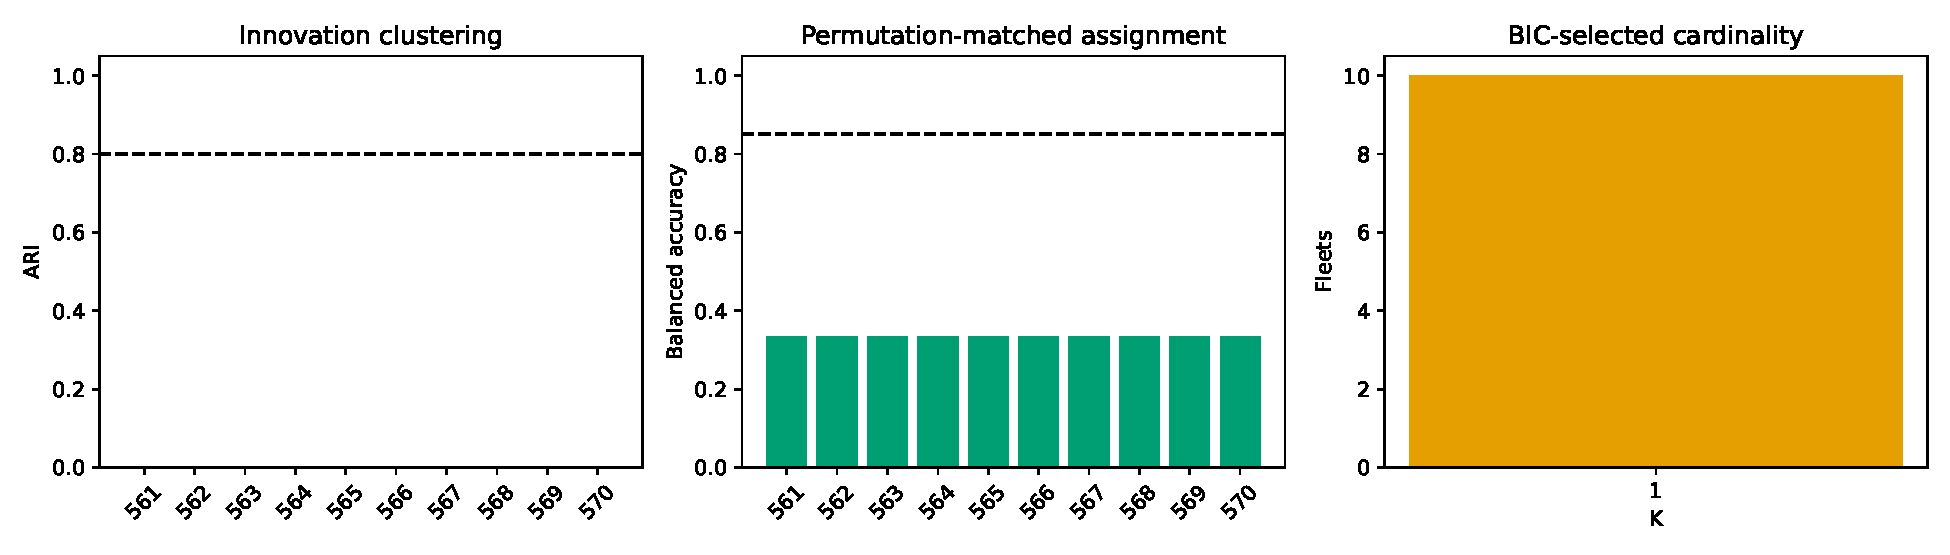
\includegraphics[width=0.98\linewidth]{../results/figures/experiment_10he_innovation_separability.pdf}
\caption{Development ARI, permutation-matched balanced accuracy, and
BIC-selected group count for leakage-safe innovation clustering.}
\label{fig:experiment10he}
\end{figure}

\paragraph{Interpretation and decision.}
The nominal observer's innovation process contains some class information,
but the aggregate signature is not a reliable stand-alone initializer for a
three-component EM algorithm. The failure is not caused by access to hidden
parameters: none enters the grouping pipeline. Instead, restricted excitation,
sensor bias, speed-block variation, and the common observer compress different
physical mismatches into partially overlapping innovation statistics.

The development gate fails and confirmation is not opened. This result does
not rule out joint state--parameter EM. It rules out using one-shot clustering
of hand-designed aggregate innovations as its sole initialization. A stronger
next test should compare complete trajectory likelihoods under several
deliberately diverse candidate physical models, or initialize a joint
structured EM with multiple restarts and allow likelihood-based soft
memberships to evolve together with the group models. Those candidate models
must be fixed design hypotheses or learned from outputs; they must not be
constructed from the clients' hidden physical parameters.

\paragraph{Reproducibility.}
Configuration and implementation are in
\path{code/config/experiment_10he.json} and
\path{code/experiments/experiment_10he_innovation_separability.py}.
Client assignments, candidate BIC values, fixed-$K$ retrospective diagnostics,
failed gate decisions, reserved confirmation seeds, leakage declaration, and
provenance hashes are stored under \path{results}.
